% !TeX root = ../main.tex
\documentclass[./../main.tex]{subfiles}

\begin{document}

Hệ thống UETWork có 2 service chính: User Service và Internship Service. Mỗi service có nhiệm vụ tự quản lý dữ liệu của mình. Dưới đây là lược đồ cơ sở dữ liệu cho 2 service này.

\subsection{Cơ sở dữ liệu của User Service (User DB)}

Hình \ref{fig:user_db_design} mô tả các bảng và mối quan hệ giữa chúng trong User DB. Bảng \ref{tab:db_roles} đến \ref{tab:db_partner_orgs} mô tả cụ thể hơn về nội dung từng bảng trong User DB.

\begin{figure}
	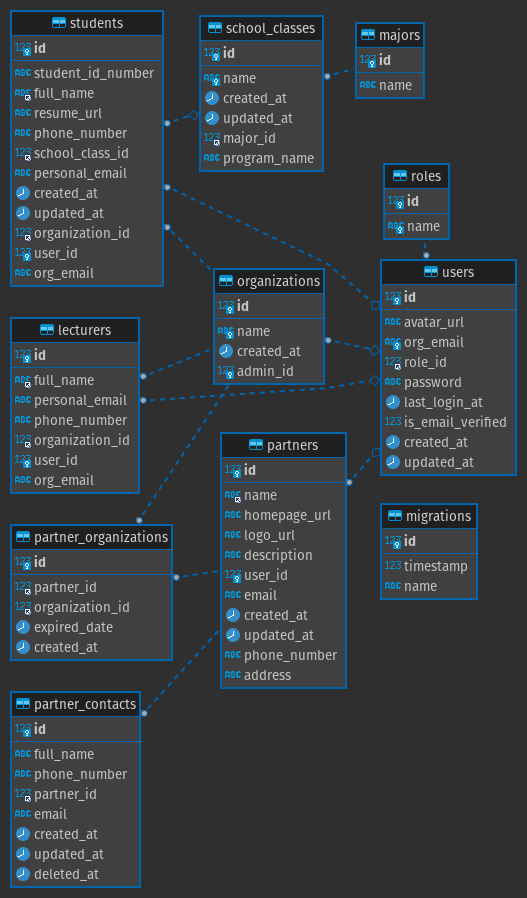
\includegraphics[width=\linewidth]{./images/image3.png}
	\caption{Lược đồ User DB}
	\label{fig:user_db_design}
\end{figure}

\begin{table}[H]
	\caption[Bảng roles]{Bảng \textbf{roles} - chứa thông tin về các role (vai trò)}
	\label{tab:db_roles}
	\begin{tabular}{|l|l|l|}
	\hline
	\textbf{Tên cột} & \textbf{Kiểu dữ liệu} & \textbf{Mô tả} \\ \hline
	id               & int                   & Mã định danh   \\ \hline
	name             & varchar               & Tên của role   \\ \hline
	phone\_number    & varchar               & Số điện thoại  \\ \hline
	\end{tabular}
\end{table}

\begin{table}[H]
	\caption[Bảng users]{Bảng \textbf{users} - chứa thông tin về tài khoản người dùng}
	\label{tab:db_users}
	\begin{tabularx}{\textwidth}{|l|l|X|}
	\hline
	\textbf{Tên cột}    & \textbf{Kiểu dữ liệu} & \textbf{Mô tả}                                         \\ \hline
	id                  & int                   & Mã định danh                                           \\ \hline
	avatar\_url         & varchar               & Địa chỉ avatar của người dùng                          \\ \hline
	org\_email          & varchar               & Địa chỉ email để người dùng đăng nhập                  \\ \hline
	role\_id            & int                   & Mã định danh của role                                  \\ \hline
	password            & varchar               & Mật khẩu đã được băm bằng thuật toán bcrypt            \\ \hline
	last\_login\_at     & timestamp             & Thời gian đăng nhập thành công gần nhất của người dùng \\ \hline
	is\_email\_verified & boolean               & Email người dùng đã được xác nhận hay chưa?            \\ \hline
	created\_at         & timestamp             & Thời gian tạo                                          \\ \hline
	updated\_at         & timestamp             & Thời gian cập nhật gần nhất                            \\ \hline
	\end{tabularx}
\end{table}

\begin{table}[H]
	\caption[Bảng organizations]{Bảng \textbf{organizations} - chứa thông tin về các khoa}
	\label{tab:db_organizations}
	\begin{tabular}{|l|l|l|}
	\hline
	\textbf{Tên cột} & \textbf{Kiểu dữ liệu} & \textbf{Mô tả}                      \\ \hline
	id               & int                   & Mã định danh                        \\ \hline
	name             & varchar               & Tên khoa                            \\ \hline
	admin\_id        & int                   & Mã định danh của quản trị viên khoa \\ \hline
	created\_at      & timestamp             & Thời gian tạo                       \\ \hline
	\end{tabular}
\end{table}

\begin{table}[H]
	\caption[Bảng school\_classes]{Bảng \textbf{school\_classes} - chứa thông tin về lớp khóa học}
	\label{tab:db_school_classes}
	\begin{tabular}{|l|l|l|}
	\hline
	\textbf{Tên cột} & \textbf{Kiểu dữ liệu} & \textbf{Mô tả}           \\ \hline
	id               & int                   & Mã định danh             \\ \hline
	name             & varchar               & Tên lớp khóa học         \\ \hline
	program\_name    & varchar               & Tên chương trình đào tạo \\ \hline
	\end{tabular}
\end{table}

\begin{table}[H]
	\caption[Bảng students]{Bảng \textbf{students} - chứa thông tin về profile sinh viên}
	\label{tab:db_students}
	\begin{tabularx}{\textwidth}{|l|l|X|}
	\hline
	\textbf{Tên cột}    & \textbf{Kiểu dữ liệu} & \textbf{Mô tả}                        \\ \hline
	id                  & int                   & Mã định danh                          \\ \hline
	student\_id\_number & varchar               & Mã số sinh viên (được nhà trường cấp) \\ \hline
	full\_name          & varchar               & Họ tên đầy đủ                         \\ \hline
	resume\_url         & varchar               & Địa chỉ lưu trữ CV của người dùng     \\ \hline
	phone\_number       & varchar               & Số điện thoại của người dùng          \\ \hline
	school\_class\_id   & int                   & Mã định danh lớp học của sinh viên    \\ \hline
	personal\_email     & varchar               & Địa chỉ email cá nhân của sinh viên   \\ \hline
	created\_at         & timestamp             & Thời gian tạo                         \\ \hline
	updated\_at         & timestamp             & Thời gian cập nhật gần nhất           \\ \hline
	organization\_id    & int                   & Mã định danh khoa của sinh viên       \\ \hline
	user\_id            & int                   & Mã định danh tài khoản                \\ \hline
	org\_email          & varchar               & Email VNU                             \\ \hline
	\end{tabularx}%
\end{table}

\begin{table}[H]
	\caption[Bảng lecturers]{Bảng \textbf{lecturers} - chứa thông tin về profile giảng viên}
	\label{tab:db_lecturers}
	\begin{tabular}{|l|l|l|}
	\hline
	\textbf{Tên cột} & \textbf{Kiểu dữ liệu} & \textbf{Mô tả}          \\ \hline
	id               & int                   & Mã định danh            \\ \hline
	full\_name       & varchar               & Họ tên đầy đủ           \\ \hline
	org\_email       & varchar               & Địa chỉ email VNU       \\ \hline
	personal\_email  & varchar               & Địa chỉ email cá nhân   \\ \hline
	phone\_number    & varchar               & Số điện thoại           \\ \hline
	organization\_id & int                   & Mã định danh khoa       \\ \hline
	user\_id         & int                   & Mã định danh người dùng \\ \hline
	\end{tabular}%
\end{table}

\begin{table}[H]
	\caption[Bảng partners]{Bảng \textbf{partners} - chứa thông tin về profile công ty trong hệ thống}
	\label{tab:db_partners}
	\begin{tabularx}{\textwidth}{|l|l|X|}
	\hline
	\textbf{Tên cột} & \textbf{Kiểu dữ liệu} & \textbf{Mô tả}                               \\ \hline
	id               & int                   & Mã định danh                                 \\ \hline
	name             & varchar               & Tên công ty                                  \\ \hline
	homepage\_url    & varchar               & Địa chỉ trang chủ công ty                    \\ \hline
	logo\_url        & varchar               & Địa chỉ logo công ty                         \\ \hline
	description      & varchar               & Mô tả công ty                                \\ \hline
	user\_id         & int                   & Mã định danh người dùng                      \\ \hline
	email            & varchar               & Địa chỉ email của bộ phận tuyển dụng công ty \\ \hline
	created\_at      & timestamp             & Thời gian tạo                                \\ \hline
	updated\_at      & timestamp             & Thời gian cập nhật gần nhất                  \\ \hline
	phone\_number    & varchar               & Số điện thoại                                \\ \hline
	address          & varchar               & Địa chỉ công ty                              \\ \hline
	org\_email       & varchar               & Email VNU                                    \\ \hline
	\end{tabularx}
\end{table}

\begin{table}[H]
	\caption[Bảng partner\_contacts]{Bảng \textbf{partner\_contacts} - chứa thông tin về liên hệ của đối tác}
	\label{tab:db_partner_contacts}
	\begin{tabular}{|l|l|l|}
	\hline
	\textbf{Tên cột} & \textbf{Kiểu dữ liệu} & \textbf{Mô tả}              \\ \hline
	id               & int                   & Mã định danh                \\ \hline
	full\_name       & varchar               & Họ tên đầy đủ               \\ \hline
	phone\_number    & varchar               & Số điện thoại               \\ \hline
	partner\_id      & int                   & Mã định danh công ty        \\ \hline
	email            & varchar               & Địa chỉ email của liên hệ   \\ \hline
	created\_at      & timestamp             & Thời gian tạo               \\ \hline
	updated\_at      & timestamp             & Thời gian cập nhật gần nhất \\ \hline
	deleted\_at      & timestamp             & Thời gian liên hệ bị xóa    \\ \hline
	\end{tabular}
\end{table}

\begin{table}[H]
	\caption[Bảng partner\_organizations]{Bảng \textbf{partner\_organizations} - chứa trạng thái liên kết giữa công ty và khoa}
	\label{tab:db_partner_orgs}
	\begin{tabular}{|l|l|l|}
	\hline
	\textbf{Tên cột} & \textbf{Kiểu dữ liệu} & \textbf{Mô tả}                       \\ \hline
	id               & int                   & Mã định danh                         \\ \hline
	partner\_id      & int                   & Mã định danh công ty                 \\ \hline
	organization\_id & int                   & Mã định danh khoa                    \\ \hline
	expired\_date    & date                  & Thời gian kết thúc hợp đồng liên kết \\ \hline
	created\_at      & timestamp             & Thời gian tạo                        \\ \hline
	\end{tabular}
\end{table}

Bảng \textbf{migrations} chứa thông tin liên quan đến migration của cơ sở dữ liệu. Không liên quan tới chức năng của hệ thống

\subsection{Cơ sở dữ liệu của Internship Service}

Hình \ref{fig:internship_db_design} mô tả thiết kế của Internship DB. Cơ sở dữ liệu này đã nhân bản lại một số bảng từ User DB để giúp việc query dễ dàng hơn. Các bảng được nhân bản từ User DB bao gồm:

\begin{itemize}
\item
  
  Bảng students
  
\item
  
  Bảng lecturers
  
\item
  
  Bảng partners
  
\item
  
  Bảng partner\_contacts
  
\item
  
  Bảng organizations
  
\item
  
  Bảng partner\_organizations
  
\item
  
  Bảng school\_classes
  
\end{itemize}

Bảng \ref{tab:db_terms} đến \ref{tab:db_posts} mô tả nội dung cụ thể của từng bảng trong cơ sở dữ liệu Internship DB.

\begin{figure}
	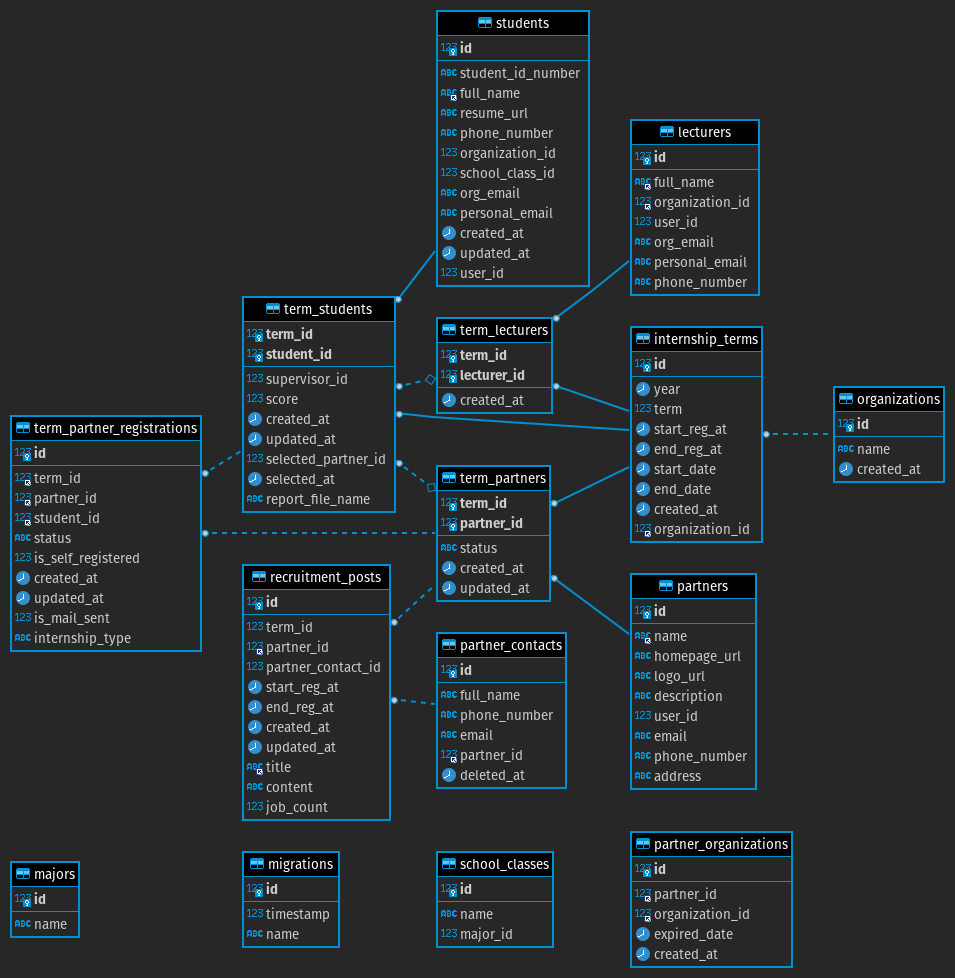
\includegraphics[width=\linewidth]{./images/image1.png}
	\caption{Lược đồ Internship DB}
	\label{fig:internship_db_design}
\end{figure}

\begin{table}[H]
	\caption[Bảng internship\_terms]{Bảng \textbf{internship\_terms} - chứa kỳ thực tập của các khoa}
	\label{tab:db_terms}
	\begin{tabular}{|l|l|l|}
	\hline
	\textbf{Tên cột} & \textbf{Kiểu dữ liệu} & \textbf{Mô tả}                     \\ \hline
	id               & int                   & Mã định danh                       \\ \hline
	year             & year                  & Năm của kỳ thực tập                \\ \hline
	term             & int                   & Đợt của kỳ thực tập (v.d. 1, 2, 3) \\ \hline
	start\_reg\_at   & timestamp             & Thời gian bắt đầu đăng ký          \\ \hline
	end\_reg\_at     & timestamp             & Thời gian kết thúc đăng ký         \\ \hline
	start\_date      & date                  & Ngày bắt đầu kỳ thực tập           \\ \hline
	end\_date        & date                  & Ngày kết thúc kỳ thực tập          \\ \hline
	created\_at      & timestamp             & Thời gian tạo                      \\ \hline
	organization\_id & int                   & Mã định danh khoa                  \\ \hline
	\end{tabular}
\end{table}

\begin{table}[H]
	\caption[Bảng term\_students]{Bảng \textbf{term\_students} - chứa thông tin thực tập của toàn bộ sinh viên}
	\label{tab:db_term_students}
	\begin{tabular}{|l|l|l|}
	\hline
	\textbf{Tên cột}      & \textbf{Kiểu dữ liệu} & \textbf{Mô tả}                       \\ \hline
	term\_id              & int                   & Mã định danh kỳ thực tập             \\ \hline
	student\_id           & int                   & Mã định danh sinh viên               \\ \hline
	supervisor\_id        & int                   & Mã định danh giảng viên hướng dẫn    \\ \hline
	score                 & int                   & Điểm                                 \\ \hline
	created\_at           & timestamp             & Thời gian tạo                        \\ \hline
	updated\_at           & timestamp             & Thời gian cập nhật gần nhất          \\ \hline
	selected\_partner\_id & int                   & Mã định danh công ty được chọn       \\ \hline
	selected\_at          & timestamp             & Thời gian chọn công ty               \\ \hline
	report\_file\_name    & varchar               & Địa chỉ lưu trữ file báo cáo cuối kỳ \\ \hline
	\end{tabular}
\end{table}



\begin{table}[H]
	\caption[Bảng term\_lecturers]{Bảng \textbf{term\_lecturers} - chứa thông tin thực tập của giảng viên}
	\label{tab:db_term_lecturers}
	\begin{tabular}{|l|l|l|}
	\hline
	\textbf{Tên cột} & \textbf{Kiểu dữ liệu} & \textbf{Mô tả}           \\ \hline
	term\_id         & int                   & Mã định danh kỳ thực tập \\ \hline
	lecturer\_id     & int                   & Mã định danh giảng viên  \\ \hline
	created\_at      & timestamp             & Thời gian tạo            \\ \hline
	\end{tabular}
\end{table}


\begin{table}[H]
	\caption[Bảng term\_partners]{Bảng \textbf{term\_partners} - chứa thông tin của công ty trong kỳ thực tập}
	\label{tab:db_term_partners}
	\begin{tabularx}{\textwidth}{|l|X|X|}
	\hline
	\textbf{Tên cột} & \textbf{Kiểu dữ liệu}                   & \textbf{Mô tả}                                               \\ \hline
	term\_id         & int                                     & Mã định danh kỳ thực tập                                     \\ \hline
	partner\_id      & int                                     & Mã định danh công ty                                         \\ \hline
	status           & enum(‘ACCEPTED', ‘PENDING', ‘REJECTED’) & Trạng thái công ty (được chấp nhận / chờ duyệt / bị từ chối) \\ \hline
	created\_at      & timestamp                               & Thời gian tạo                                                \\ \hline
	updated\_at      & timestamp                               & Thời gian cập nhật gần nhất                                  \\ \hline
	\end{tabularx}
\end{table}


\begin{table}[H]
	\caption[Bảng term\_partner\_registrations]{Bảng \textbf{term\_partner\_registrations} - chứa thông tin đăng ký thực tập của sinh viên}
	\label{tab:db_term_partner_regs}
	\begin{tabularx}{\textwidth}{|l|X|X|}
	\hline
	\textbf{Tên cột}     & \textbf{Kiểu dữ liệu}                           & \textbf{Mô tả}                                 \\ \hline
	id                   & int                                             & Mã định danh                                   \\ \hline
	term\_id             & int                                             & Mã định danh kỳ thực tập                       \\ \hline
	student\_id          & int                                             & Mã định danh sinh viên                         \\ \hline
	partner\_id          & int                                             & Mã định danh công ty                           \\ \hline
	status               & enum(‘PASSED', ‘FAILED', ‘SELECTED', ‘WAITING') & Kết quả phỏng vấn                              \\ \hline
	is\_self\_registered & boolean                                         & Có phải sinh viên này đã tự đăng ký không?     \\ \hline
	created\_at          & timestamp                                       & Thời gian tạo                                  \\ \hline
	updated\_at          & timestamp                                       & Thời gian cập nhật gần nhất                    \\ \hline
	is\_mail\_sent       & boolean                                         & Mail thông báo đã được gửi hay chưa?           \\ \hline
	internship\_type     & enum(‘ASSOCIATE’, ‘OTHER')                      & Loại thực tập (thực tập đối tác/công ty ngoài) \\ \hline
	\end{tabularx}
\end{table}

\begin{table}[H]
	\caption[Bảng recruitment\_posts]{Bảng \textbf{recruitment\_posts} - chứa bài đăng tuyển dụng trong 1 kỳ thực tập}
	\label{tab:db_posts}
	\begin{tabular}{|l|l|l|}
	\hline
	\textbf{Tên cột}     & \textbf{Kiểu dữ liệu} & \textbf{Mô tả}                   \\ \hline
	id                   & int                   & Mã định danh                     \\ \hline
	term\_id             & int                   & Mã định danh kỳ thực tập         \\ \hline
	partner\_id          & int                   & Mã định danh công ty             \\ \hline
	partner\_contact\_id & int                   & Mã định danh liên hệ của đối tác \\ \hline
	start\_reg\_at       & timestamp             & Ngày bắt đầu đăng ký             \\ \hline
	end\_reg\_at         & timestamp             & Ngày kết thúc đăng ký            \\ \hline
	title                & varchar               & Tiêu đề bài đăng                 \\ \hline
	content              & varchar               & Nội dung bài đăng                \\ \hline
	job\_count           & int                   & Số người cần tuyển               \\ \hline
	\end{tabular}
\end{table}

\end{document}
